\scanpage{25}
\figure{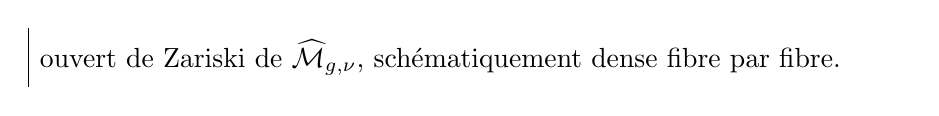
\begin{tikzpicture}
\node[anchor=north west,text width=0.9\linewidth,align=left,inner sep=4pt] (T) at (0,0) {
ouvert de Zariski de $\widehat{\mathcal M}_{g,\nu}$, schématiquement dense fibre par fibre.
};
\draw[line width=0.5pt] (T.north west)--(T.south west);
\end{tikzpicture}}

On en déduit aisément p.ex. la connexité des fibres géom. de $\mathcal M_{g,\nu}$ en toute car., à partir de \deleted{\unsure{la}} \unsure{connexité} en car. $0$. D'autre part, pour $\forall$ type $[G]$ de MD-graphe, ayant le type numérique $(g,\nu)$, les courbes \unsure{standard|standart} de type $[G]$ (sur une base quelc. $\mathcal S$) sont manifestement des MD-courbes relatives de type numérique $(g,\nu)$. On en conclut un morphisme canonique
\[
(25)\qquad\mathcal M_{[G]}\hookrightarrow\widehat{\mathcal M}_{g,\nu}
\]
dont on vérifie aisément que c'est une \uline{immersion}. Le cas où $G$ est le
\mspage{24}
